\documentclass[10pt,a4paper]{article}
\usepackage[utf8]{inputenc}
\usepackage{amsmath}
\usepackage{amsfonts}
\usepackage{amssymb}
\usepackage{titlesec}
\usepackage{graphicx}
\usepackage{float} 
\usepackage{subcaption}
\usepackage[left=2cm,right=2cm,top=2cm,bottom=2cm]{geometry}
\usepackage[numbers]{natbib}

\begin{document}

\title{MRI image reconstruction using fastMRI library \\ \vspace{0.5cm} \large Summary}
\author{Dražen Bertić}
\date{Osijek, 2023} % Or any specific date

\maketitle

\section{fastMRI}

fastMRI is a collaborative exploratory project by Facebook AI Research with the goal of developing faster ways of MRI image acquisition. It consists of datasets of brain and knee MRI images, and of code repository with tools to work with dataset and model implementation. \cite{zbontar2019fastmri}

\subsection{Models in fastMRI library}

\subsubsection{Zero-Filled}

The zero-fill method inserts zeros in the places of the uncollected k-space data points. It expands the undersampled k-space data to the size needed for a full-resolution image, but with zeros where we lack actual data. After zero-filling the k-space inverse Fourier transform is applied to convert data back to the spatial domain.

\subsubsection{Compressed Sensing}

Compressed Sensing is based on a mathematical principal which states that images and signals can be represented with fewer data without losing a significant amount of information. The implementation in fastMRI uses BART (The Berkeley Advanced Reconstruction Toolbox) which is a free and open-source image-reconstruction framework for Computational Magnetic Resonance Imaging. 

\subsubsection{U-Net}

The U-Net model provided by fastMRI is designed for single-coil image reconstruction but can be adapted to multi-coil images using the zero-fill method for each coil. The model consists of two main paths: a encoder path and decoder path. Encoder paths goal is context and content capture using 3x3 convolutions, instance normalization, ReLU activation and max-pooling down-sampling. Decoder path is used for spatial localization and block up-scaleing. Both paths are connected with skip connections which enchance detail and precision in the output using high-resolution features. \cite{ronneberger2015unet} \cite{zbontar2019fastmri}

\begin{figure}[H]
\centering
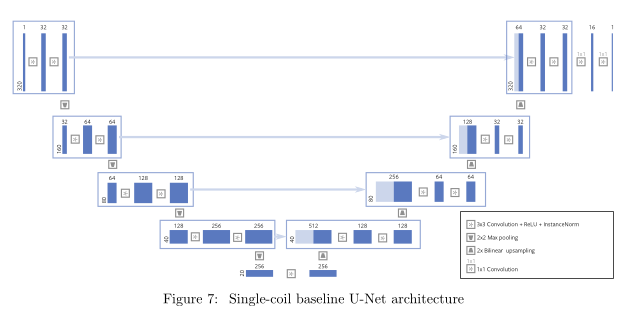
\includegraphics[scale=0.5]{images/unet-architecture.png}
\caption{U-Net Architecture \cite{zbontar2019fastmri}}
\end{figure}

\newpage
\subsubsection{End-to-End VarNet}

End-to-End Varnet model is designed to learn complete process of reconstruction. End-to-End means we can give it raw data without any preprocessing and it will give out processed result. \cite{sriram2020endtoend}

It takes multi coil k-space as input and applies a series of refinement steps which we call cascades. At the begginning sensitivity maps are estimated using SME module. In each cascade Data Consistency module (DC) and Refinement module (R) is applied. After cascades, IFT is performed to get image from each k-space, followed by root-sum-squares reduction (RSS) for each pixel. Image is then cropped and output is given. \cite{sriram2020endtoend}

\paragraph{SME Module}

Sensitivity Map Estimation module estimates sensitivity maps which are later used in Refinement module. In traditional VarNet sensitivity maps are computed using the ESPIRiT algorithm, but here they're computed using SME module:

$$ H = dSS \circ CNN \circ \mathcal{F}^{-1} \circ M_{\text{center}} $$


\begin{itemize}
  \item $M_{\text{center}}$ zeroes all lines except ACS lines. ACS are autocalibration lines, the central region of k-space corresponding to low frequencies which is used for sensitivity estimation.
  \item CNN is a convolutional neural network. It is the same as the one used in cascades (U-Net), except with fewer channels and fewer parameters.
  \item dSS normalizes sensitivity maps. They need to satisfy the equation below:
\end{itemize}

\paragraph{DC Module}

Data Consistency computes correction map which brings the intermediate k-space closer to the measured k-space values. It performs subtraction between inputs and identifies differences between them. After that, it applies a correction map to differences identified in the previous step. Adjusting intermediate k-space so it becomes more consistent with measured k-space values.

\paragraph{Refinement Module}

The refinement module maps multi-coil k-space data into one image. It takes intermediate k-space and estimated sensitivity maps (ESM) as input. Applies IFT to intermediate k-space, then using ESM it reduces it to a single image. It applies U-Net on the image and then, using ESM, expands them to images seen by each coil. After all of those steps, it applies FT so output is k-space.

\begin{figure}[H]
\centering
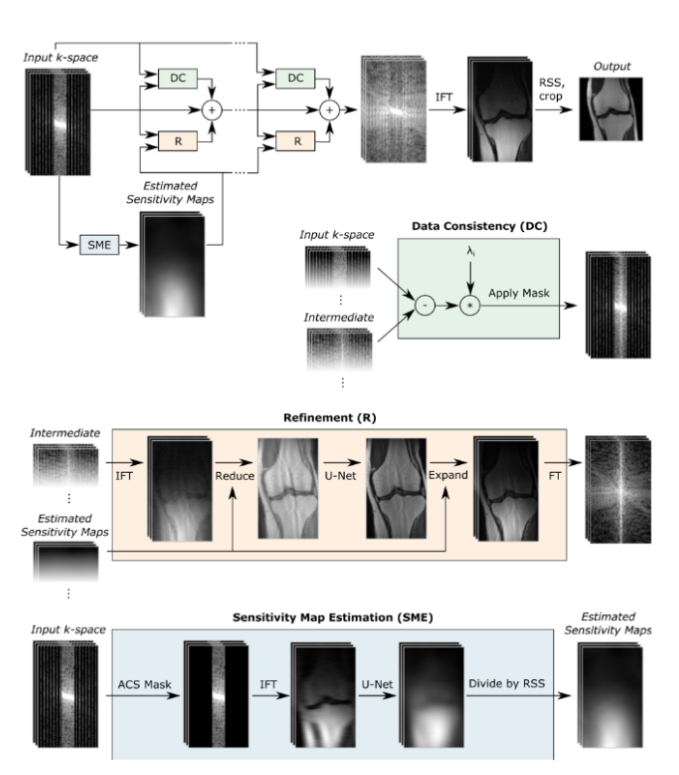
\includegraphics[scale=0.5]{images/e2e-varnet-architecture.png}
\caption{End-to-End VarNet Architecture \cite{sriram2020endtoend}}
\end{figure}

\subsection{Results}

\begin{figure}[H]
\centering
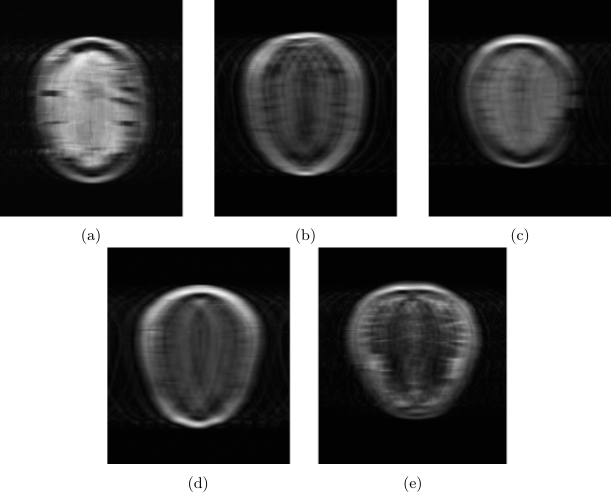
\includegraphics[width=400pt]{./images/test-images.png}
\caption{Test images a) AXFLAIR, b) AXT1, c) AXT1PRE, d) AXT1POST i d) AXT2}
\end{figure}

\begin{figure}[H]
\centering
\begin{minipage}{.45\textwidth}
  \centering
  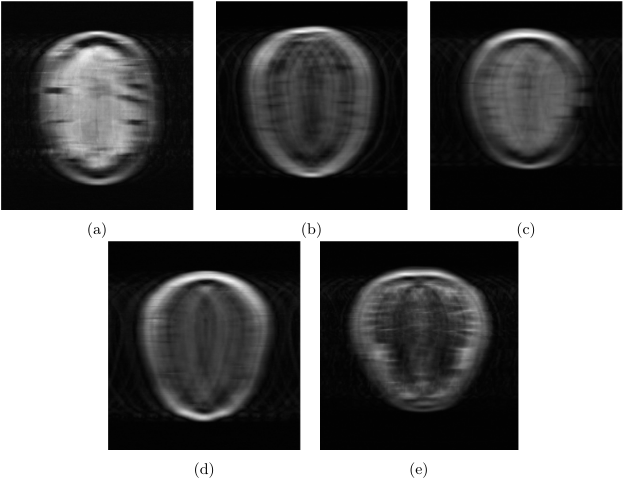
\includegraphics[width=200pt]{./images/zero-fill.png}
  \caption{Zero-fill a) AXFLAIR, b) AXT1, c) AXT1PRE, d) AXT1POST i d) AXT2}
\end{minipage}%
\hspace{20pt} % Space between the two images
\begin{minipage}{.45\textwidth}
  \centering
  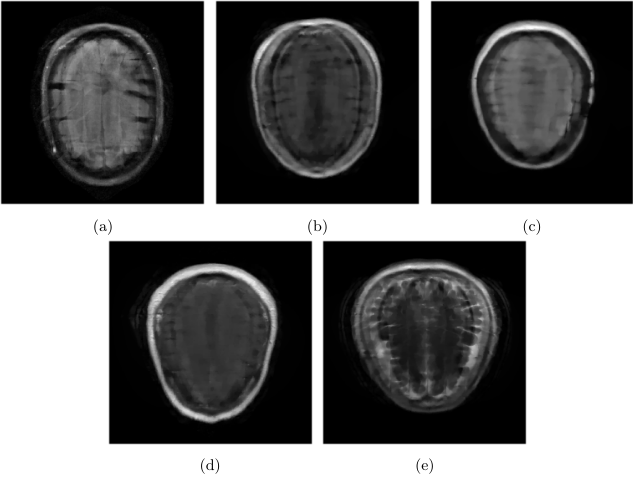
\includegraphics[width=200pt]{./images/compressed-sensing-images.png}
  \caption{Compressed Sensing a) AXFLAIR, b) AXT1, c) AXT1PRE, d) AXT1POST i d) AXT2}
\end{minipage}

\vspace{20pt} % Space between the two rows of images

\begin{minipage}{.45\textwidth}
  \centering
  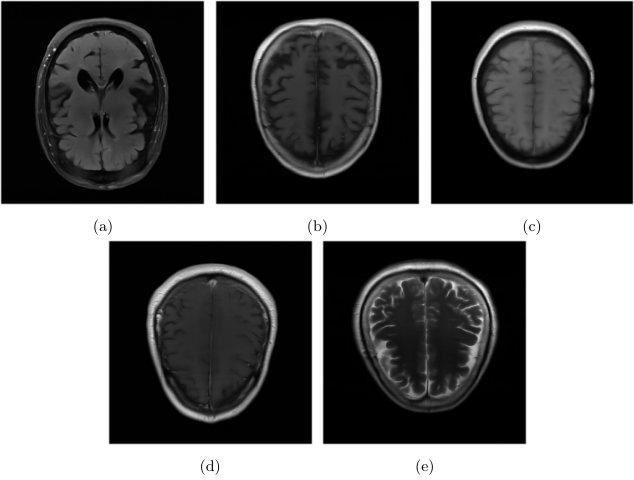
\includegraphics[width=200pt]{./images/unet-images.png}
  \caption{U-Net a) AXFLAIR, b) AXT1, c) AXT1PRE, d) AXT1POST i d) AXT2}
\end{minipage}%
\hspace{20pt} % Space between the two images
\begin{minipage}{.45\textwidth}
  \centering
  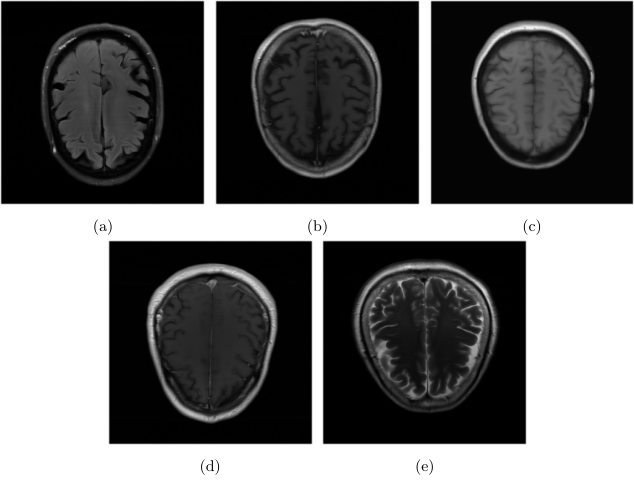
\includegraphics[width=200pt]{./images/varnet-images.png}
  \caption{End-to-End VarNet a) AXFLAIR, b) AXT1, c) AXT1PRE, d) AXT1POST i d) AXT2}
\end{minipage}
\end{figure}

\newpage

\section{Current state-of-art}

For a long time End-to-End VarNet presented best results on fastMRI bechmark, but in March 2023 HUMUS-Net network which outperforms End-to-End VarNet has been presented. It's an unrolled, transformer-convolutional hybrid network for accelerated MRI reconstruction. Architecture consists of a sequence of sub-networks (cascades). Each cascade represents an unrolled iteration of an underlying optimization algorithm in k-space with an image-domain denoiser, the HUMUS-Block. The HUMUS-Block acts as an image-space denoiser that receives an intermediate reconstruction from the previous cascade and performs a single step of denoising to produce an improved reconstruction for the next cascade. It extracts high-resolution, shallow features and low-resolution, deep features through a novel multi-scale transformer-based block, and synthesizes high-resolution features from those. Limitation of current architecture is that it required fixed-size inputs. \cite{fabian2023humusnet}

\begin{figure}[H]
\centering
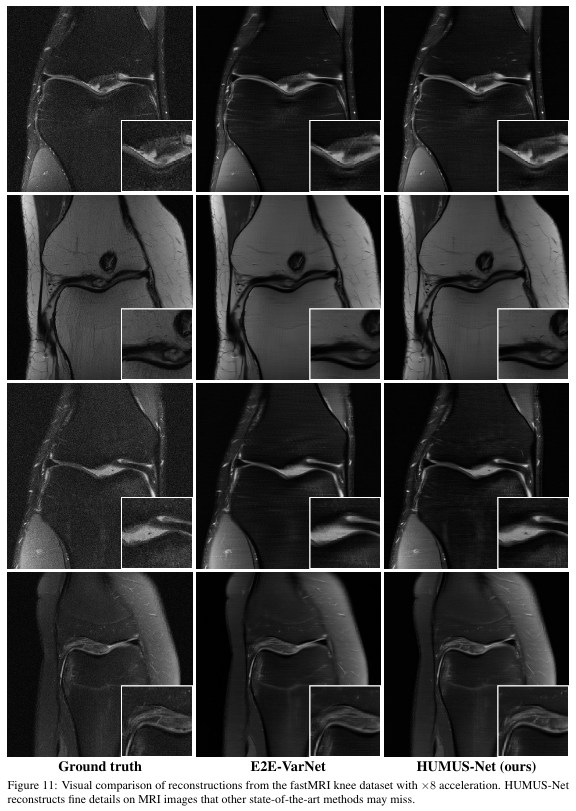
\includegraphics[width=300pt]{./images/humus-comparison.png}
\caption{Humus results comparison \cite{fabian2023humusnet}}
\end{figure}

\begin{figure}[H]
\centering
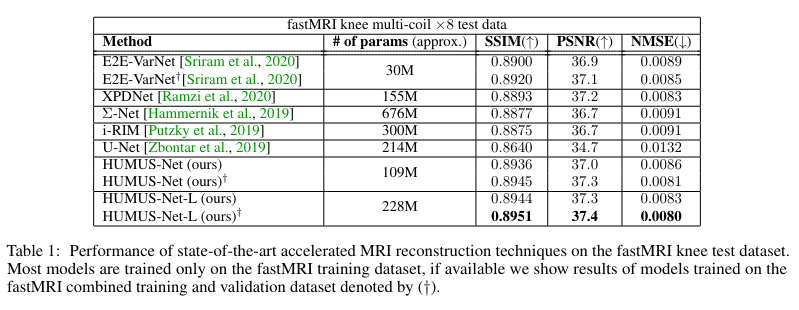
\includegraphics[width=400pt]{./images/humus-perf.png}
\caption{Humus performance comparison \cite{fabian2023humusnet}}
\end{figure}

\section{Conclusion}

FastMRI library provides set of tools, models and dataset needed to work on MRI reconstruction. Techniques it provides are zero-fill, compressed sensing, U-Net and End-to-End VarNet. For a long time End-to-End VarNet presented best results, until HUMUS-Net, which brought better results, was presented in March 2023. But still, reconstructions are still now clinicaly valid because of their total lack of details. Even if they were, they would need a approval of medical experts and couldn't be used in real diagnostics.

\section{Master thesis}

Goal is to implement modified U-Net and VarNet models and adapt them for the task of reconstructing MRI brain images. The display, explain and compare the results and determine the accuracy of the developed system.

\newpage
\bibliographystyle{plainnat} % Or any other style you prefer
\bibliography{references}    % Assumes your BibTeX file is 'references.bib'

\end{document}
